\subsection{Pepper Noise}\label{image_1}
Pepper noise is when a set of pixels on an image are complete black, without the actual photographed scene has these elements.
To find the noise in an image, an uniform area is selected and analyzed.
In figure \ref{fig:hist_pepper} can it be seen that the image suffers from pepper noise.
It is assumed that the amount of pepper in the uniform is the same all over the image.

\begin{figure}[H]
\includegraphics[width = 0.4 \textwidth]{graphics/hist.png}
\caption{Histogram of the original ``Image1.png'' showing pepper noise in a uniform area.}
\label{fig:hist_pepper}
\end{figure}

A median filter is good to combat salt and pepper noise as it takes the midpoint and thus avoids extreme values.
This assumes that the amount of salt or pepper is less than 20\% and the filter is large enough to get values which are neither entire salt or entire pepper.
To remove pepper noise from an image with mostly pepper noise, the amount of pepper damage needs to be found.
The image was detected to be 60\% pepper.
This means a median filter is not viable as the midpoint is likely to turn out as pepper.

Knowing this means that the midpoint must be shifted towards a lighter color.
This method is called alpha trimmed mean.
the new midpoint is called a quantile, which can be found in equation \ref{eq:quantile}.
The midpoint is thus chosen to be 80\%. 

\begin{equation}
 q = (\text{pepper}-\text{salt}+1)/2 \label{eq:quantile}
\end{equation}

A 3x3 midpoint filter is applied to the image to remove the majority of the damage to the image.
Then a 7x7 alpha trimmed mean with a width of 3 is applied to further remove the pepper noise.

To see if the filters does damage to the original image an area with more complex features are shown.
In figure \ref{fig:complex1_after_alpha} can the area be seen after the alpha trimmed mean filter has been applied.
It can be seen that there is still noise present in the image.

\begin{figure}[H]
\includegraphics[width = 0.4 \textwidth]{graphics/complex1_step1.png}
\caption{Image in a compex area after alpha trimmed mean filter.}
\label{fig:complex1_after_alpha}
\end{figure}

To see the noise, another histogram of the uniform area is made.
In figure \ref{fig:hist_img1_after_alpha} can the histogram of the uniformed area after the two filters be seen.
The histogram suggest that there is still Gaussian noise in the image.
Since Gaussian noise is multiplicative instead of additive, an homomorphic blurring filter is applied.
By taking the image into logarithmic space, the noise becomes additive and thus can be separated with a arithmetic mean filter.

\begin{figure}[H]
\includegraphics[width = 0.4 \textwidth]{graphics/hist1_step1.png}
\caption{Histogram of the filtered uniform area after alpha trimmed mean filter.}
\label{fig:hist_img1_after_alpha}
\end{figure}

The final image of image 1 can be seen in figure \ref{fig:final_image1}.

\begin{figure}[H]
\centering
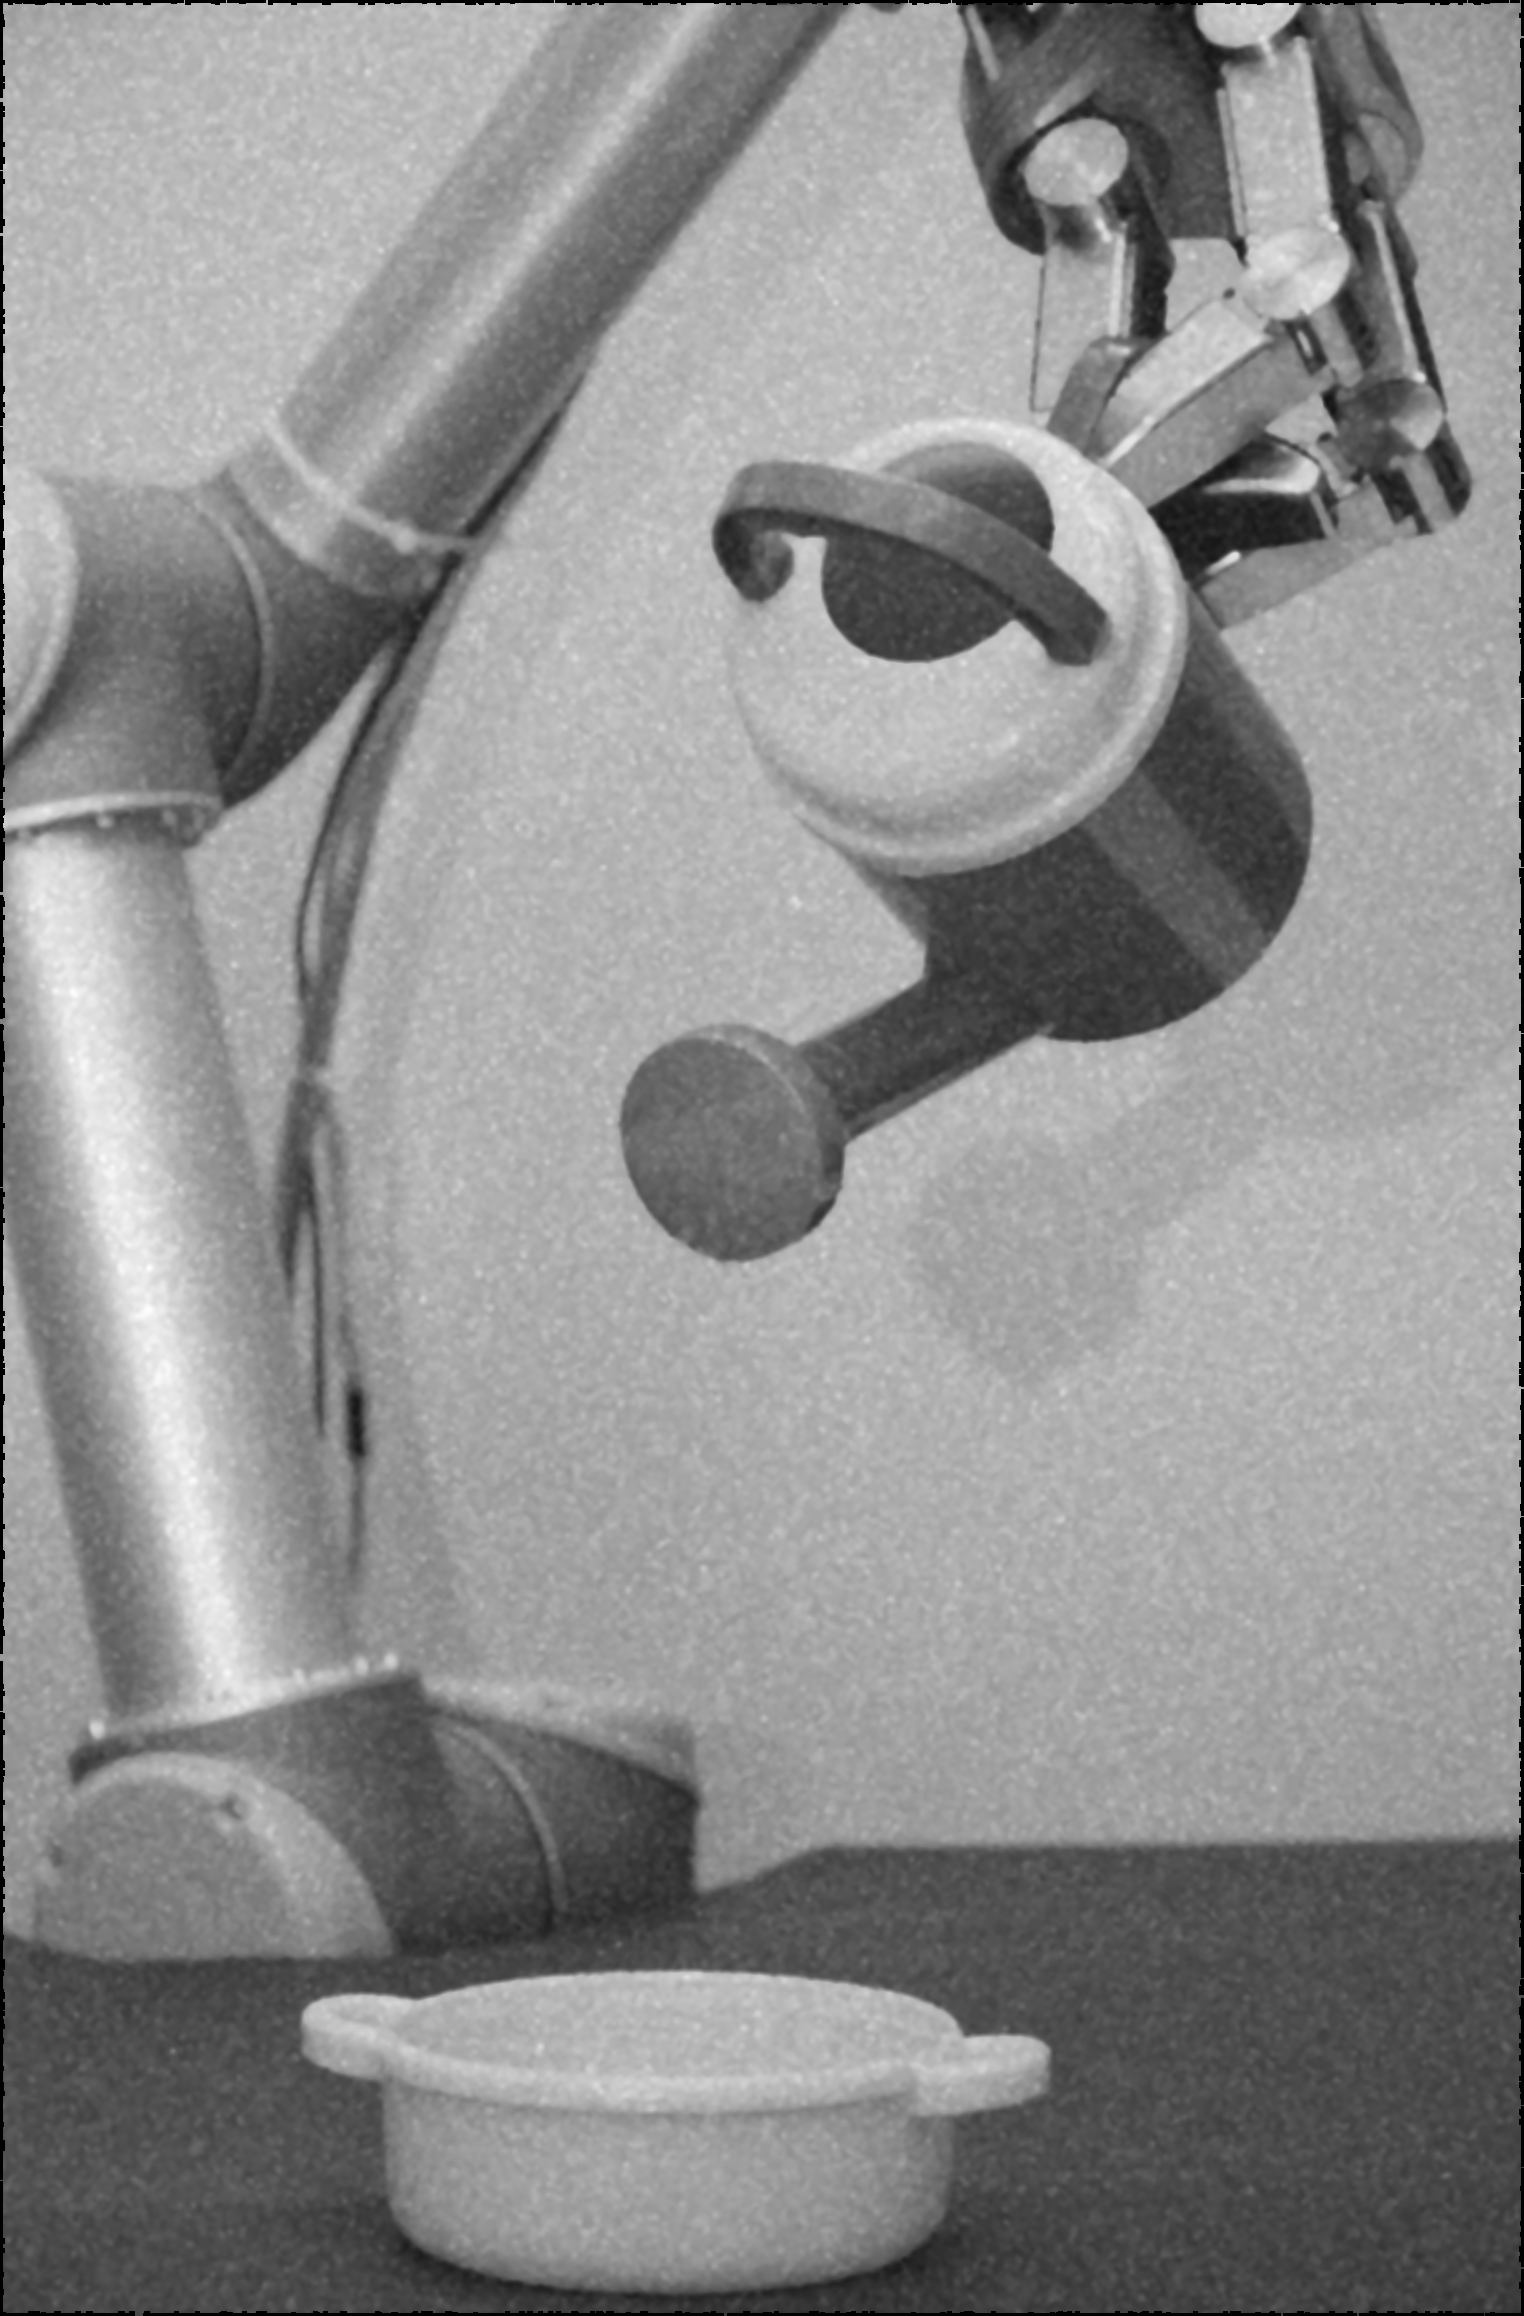
\includegraphics[width = 0.8 \linewidth]{../code/images/image_result_1.png}
\caption{Image 1 restored.}
\label{fig:final_image1}
\end{figure}
